\section{Análise gramatical}

\begin{frame}[fragile]{Análise gramatical}

    \begin{itemize}
        \item A análise gramatical é o processo de se determinar se uma cadeia de tokens pode ser gerada por uma gramática
        \pause

        \item O compilador deve ser capaz de construir uma árvore gramatical, mesmo que de forma implícita
        \pause

        \item Um analisador gramatical pode ser construído para qualquer gramática
        \pause

        \item Para qualquer gramáticas livres de contexto existe um analisador gramatical que analisa $N$ tokens com complexidade $O(N^3)$
        \pause

        \item Contudo, existem analisadores lineares para quase todas as gramáticas livres de contexto que surgem na prática
    \end{itemize}

\end{frame}

\begin{frame}[fragile]{Análise {\it top-down} e {\it bottom-up}}

    \begin{itemize}
        \item Há duas classes principais de analisadores gramaticais
        \pause

        \item Analisadores {\it top-down} a construção parte da raiz da árvore gramatical para suas folhas
        \pause

        \item Analisadores {\it bottom-up} partem das folhas em direção à raiz
        \pause

        \item Os analisadores \textit{top-down} são mais populares, pois é possível construir analisadores eficientes desta classe de forma manual
        \pause

        \item Já os analisadores \textit{bottom-up} podem manipular uma gama mais ampla de gramáticas
        \pause

        \item Geradores de analisadores gramaticais tendem a usar métodos \textit{bottom-up}
    \end{itemize}

\end{frame}

\begin{frame}[fragile]{Construção {\it top-down} de uma árvore gramatical}

    \begin{enumerate}
        \item Inicie na raiz, rotulada pelo não-terminal de partida
        \pause

        \item Repita os seguintes passos:
        \pause

        \begin{enumerate}[(a)]
            \item Para o nó $n$, rotulado pelo não-terminal $A$, selecione uma das produções para $A$ e construa os filhos de $n$ com os símbolos do lado 
            direito da produção
            \pause

            \item Encontre o próximo nó no qual uma subárvore deve ser construída
        \end{enumerate} 
    \end{enumerate}
    \pause

    \vspace{0.1in}
    Observações:
    \pause
    \begin{enumerate}[(i)]
        \item A depender da gramática, esta construção pode ser implementada com uma única passagem da entrada, da esquerda para a direita
        \pause

        \item O token que está sendo observado é frequentemente denominado \textit{lookahead}
        \pause

        \item Inicialmente \textit{lookahead} é o token mais à esquerda da entrada
    \end{enumerate}
\end{frame}

\begin{frame}[fragile]{Exemplo: gramática para geração de subtipos em Pascal}

\[
    \begin{array}{rcl}
        tipo & \to & primitivo \\
             & | & \uparrow \mathbf{id} \\
             & | & \mathbf{array}\ [\ primitivo \ ]\ \mathbf{of}\ tipo \\
        \\
        primitivo & \to & \mathbf{integer} \\
             & | & \mathbf{char} \\
             & | & \mathbf{num}\ ..\ \mathbf{num}
    \end{array}
\]
    \pause
    \vspace{0.2in}

    Observação: os dois pontos (`$..$') formam um único token. 

\end{frame}

\begin{frame}[fragile]{Exemplo de construção {\it top-down} da árvore gramatical}

    Considere a expressão \code{pascal}{array [ num .. num ] of integer}, gerada a partir da gramática de subtipos em Pascal.
    \pause

    \vspace{0.2in}

    \begin{enumerate}[(a)]
        \item A construção inicial na raiz da árvore. O rótulo da raiz é o não-terminal de partida
        \pause

        \begin{center}
           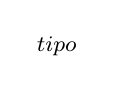
\begin{tikzpicture} 
                \node (A) at (6, 6) { \footnotesize $tipo$ };
           \end{tikzpicture} 
        \end{center}
        \pause

        \item A única produção de $tipo$ que inicia com o  \textit{lookahead} (neste momento, \code{pascal}{array}) é a terceira. Esta produção será
            usada para a criação dos filhos do nó raiz.
        \pause

        \begin{center}
           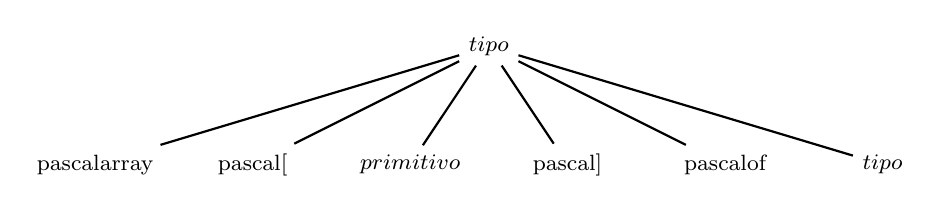
\begin{tikzpicture} 
                \node (A) at (5, 5) { \footnotesize $tipo$ };
                \node (B1) at (0, 3.5) { \footnotesize \code{pascal}{array} };
                \node (B2) at (2, 3.5) { \footnotesize \code{pascal}{[} };
                \node (B3) at (4, 3.5) { \footnotesize $primitivo$ };
                \node (B4) at (6, 3.5) { \footnotesize \code{pascal}{]} };
                \node (B5) at (8, 3.5) { \footnotesize \code{pascal}{of} };
                \node (B6) at (10, 3.5) { \footnotesize $tipo$ };

                \draw[thick] (A) to (B1);
                \draw[thick] (A) to (B2);
                \draw[thick] (A) to (B3);
                \draw[thick] (A) to (B4);
                \draw[thick] (A) to (B5);
                \draw[thick] (A) to (B6);
           \end{tikzpicture} 
        \end{center}
 
    \end{enumerate}
\end{frame}

\begin{frame}[fragile]{Exemplo de construção {\it top-down} da árvore gramatical}

    \begin{enumerate}[(a)]
        \setcounter{enumi}{2}
            \item O filho mais à esquerda tem como rótulo \code{pascal}{array}. Como este rótulo coincide com \textit{lookahead}, a construção prossegue para o
                próximo filho
            \pause

        \item \textit{Lookahead} é atualizado para \code{pascal}{[} e confrontado com o segundo filho à esquerda da raiz. Como há nova coincidência entre o rótulo
            e \textit{lookahead}, a construção prossegue
            \pause

        \item O nó seguinte contém o não-terminal $primitivo$ e \textit{lookahead} contém o token \code{pascal}{num}. Assim a terceira produção de $primitivo$
            é utilizada para gerar os novos filhos
        \pause

       \begin{center}
           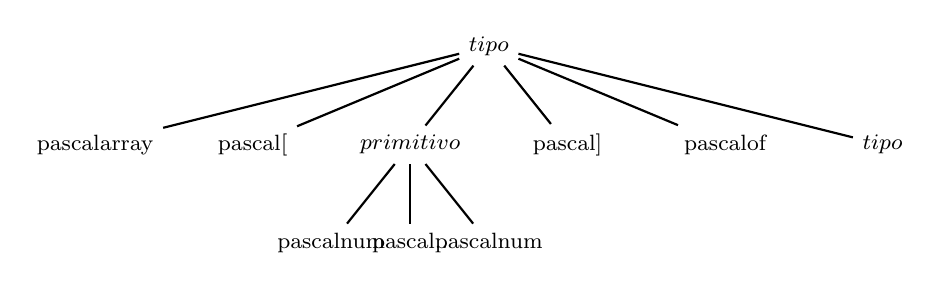
\begin{tikzpicture} 
                \node (A) at (5, 5) { \footnotesize $tipo$ };
                \node (B1) at (0, 3.75) { \footnotesize \code{pascal}{array} };
                \node (B2) at (2, 3.75) { \footnotesize \code{pascal}{[} };
                \node (B3) at (4, 3.75) { \footnotesize $primitivo$ };
                \node (B4) at (6, 3.75) { \footnotesize \code{pascal}{]} };
                \node (B5) at (8, 3.75) { \footnotesize \code{pascal}{of} };
                \node (B6) at (10, 3.75) { \footnotesize $tipo$ };
                \node (C1) at (3, 2.5) { \footnotesize \code{pascal}{num} };
                \node (C2) at (4, 2.5) { \footnotesize \code{pascal}{..} };
                \node (C3) at (5, 2.5) { \footnotesize \code{pascal}{num} };

                \draw[thick] (A) to (B1);
                \draw[thick] (A) to (B2);
                \draw[thick] (A) to (B3);
                \draw[thick] (A) to (B4);
                \draw[thick] (A) to (B5);
                \draw[thick] (A) to (B6);
                \draw[thick] (B3) to (C1);
                \draw[thick] (B3) to (C2);
                \draw[thick] (B3) to (C3);
        
           \end{tikzpicture} 
        \end{center}
 
    \end{enumerate}
\end{frame}

\begin{frame}[fragile]{Exemplo de construção {\it top-down} da árvore gramatical}

    \begin{enumerate}[(a)]
        \setcounter{enumi}{6}
        \item Os próximos tokens (\code{pascal}{:, num, of}) coincidem com os respectivos filhos
            \pause

        \item O último valor que \textit{lookahead} assum é \code{pascal}{integer}, o qual é confrontado com o filho mais à direita da raiz. Como o nó tem
            como rótulo o não-terminal $tipo$, a primeira produção deste deve ser usada para construir o novo nó, que por sua vez usa a primeira produção de
            $primitivo$ para construir seu único filho

        \pause
       \begin{center}
           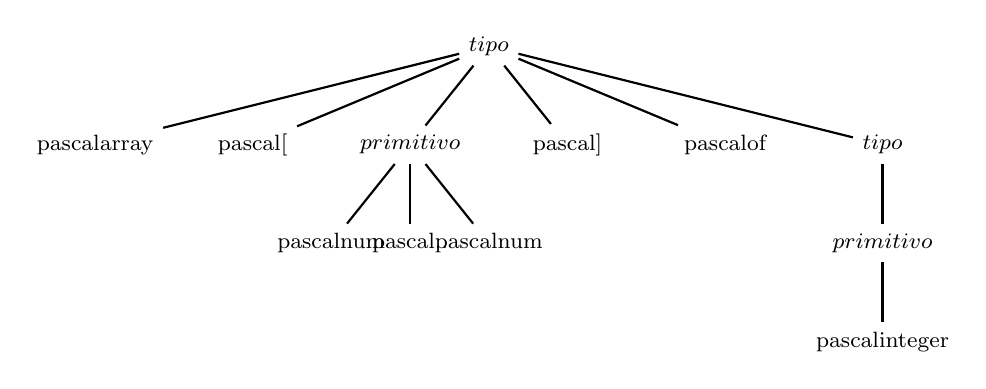
\begin{tikzpicture} 
                \node (A) at (5, 5) { \footnotesize $tipo$ };
                \node (B1) at (0, 3.75) { \footnotesize \code{pascal}{array} };
                \node (B2) at (2, 3.75) { \footnotesize \code{pascal}{[} };
                \node (B3) at (4, 3.75) { \footnotesize $primitivo$ };
                \node (B4) at (6, 3.75) { \footnotesize \code{pascal}{]} };
                \node (B5) at (8, 3.75) { \footnotesize \code{pascal}{of} };
                \node (B6) at (10, 3.75) { \footnotesize $tipo$ };
                \node (C1) at (3, 2.5) { \footnotesize \code{pascal}{num} };
                \node (C2) at (4, 2.5) { \footnotesize \code{pascal}{..} };
                \node (C3) at (5, 2.5) { \footnotesize \code{pascal}{num} };
                \node (D1) at (10, 2.5) { \footnotesize $primitivo$ };
                \node (E1) at (10, 1.25) { \footnotesize \code{pascal}{integer} };

                \draw[thick] (A) to (B1);
                \draw[thick] (A) to (B2);
                \draw[thick] (A) to (B3);
                \draw[thick] (A) to (B4);
                \draw[thick] (A) to (B5);
                \draw[thick] (A) to (B6);
                \draw[thick] (B3) to (C1);
                \draw[thick] (B3) to (C2);
                \draw[thick] (B3) to (C3);
                \draw[thick] (B6) to (D1);
                \draw[thick] (E1) to (D1);
        
           \end{tikzpicture} 
        \end{center}
 
    \end{enumerate}
\end{frame}

